%\documentclass[a4paper,10pt]{article}
\documentclass[seminar,twoside]{iitbreport}
\usepackage[utf8]{inputenc}
\usepackage{graphicx}
%\usepackage[hidelinks]{hyperref}
\usepackage{xcolor}
\hypersetup{
    hidelinks,
     colorlinks,
    linkcolor={blue!30!black},
    citecolor={blue!50!black},
    urlcolor={blue!80!black}
}

\usepackage{array}

\newcolumntype{L}[1]{>{\raggedright\let\newline\\\arraybackslash\hspace{0pt}}m{#1}}
\newcolumntype{C}[1]{>{\centering\let\newline\\\arraybackslash\hspace{0pt}}m{#1}}
\newcolumntype{R}[1]{>{\raggedleft\let\newline\\\arraybackslash\hspace{0pt}}m{#1}}

\usepackage{hhline}
\setcounter{secnumdepth}{4}
\setcounter{tocdepth}{4}
%opening
%\title{\textbf{Virtualization for embedded systems}\\M.Tech. Seminar Report}
%\author{\textbf{Sahil Singh}\\143050001\\\\\\Seminar Guide\\\textbf{Prof. Purushottam Kulkarni}\\\\\\\\\\\\Department of Computer Science and engineering\\Indian Institute of Technology Bombay\\Mumbai, Maharashtra}

\date{}

\begin{document}


\title{Virtualization for embedded systems}
\author{Sahil Singh \\ (143050001) \\  under the guidance of  \\ Prof. Purushottam Kulkarni}
%\date{\today}
\degree{M.Tech}
\dept{Computer Science and Engineering}
\monthyear{APRIL 2015}

%\makecoverpage
\maketitle

\renewcommand{\thesection}{\arabic{section}}

%\begin{abstract}
 
%\end{abstract}

\tableofcontents
\newpage
\let\LaTeXStandardClearpage\clearpage
\let\clearpage\relax
\listoftables
\listoffigures
\let\clearpage\LaTeXStandardClearpage
\newpage
\section{Introduction}
Silicon wafer fabrication technology has advanced by leaps and bounds in recent years.
This trend, driven by Moore's law, has lead to emergence of new and powerful microprocessors.
This, in turn, has fuelled the adoption of virtualization on various platforms, in an effort to make efficient use of these capable processors, and to support a variety of applications on the same platform.
\\\\
%Virtualization is also seen as a means to improve the portability of software by shielding applications from the rapid changes happening in the underlying hardware.
The embedded systems world hasn't remained untouched by these developments, and is witnessing tremendous growth in  complexity and variety of applications.
Virtualization solutions, however, for embedded platforms differ in their use-cases, and constraints, from their x86 counterparts, and hence the solutions developed for x86 platforms cannot be directly ported.
\\\\
Intel, with its low power x86 processors has a small and emerging portfolio of processors targeted towards embedded platforms.
In the course of my study I mainly focused on x86 server, and desktop processors, therefore, the term x86 mentioned in this document refers to x86 processors for desktops and servers.
 
\subsection{Virtualization}
Virtualization, as an idea originated in the 1960s. Then it was used mainly to allow multiple users to access a common, and often expensive computing platform.
With the advent of multi-user operating systems, and popularization of desktops, this was no longer needed, and virtualization lost it's significance.
During the last few decades, however virtualization has risen again, albeit with a new set of use cases.
The following are the main use cases of virtualization, and depending on the application domain, or hardware platform some may be more critical than others (For, eg. a provider of cloud services will
be more concerned about the most efficient use of hardware he owns, to maximize profit, while ensuring least discomfort to his customers, whereas for a user running multiple VMs on his/her mobile phone, battery life might
be a primary concern) .
\begin{itemize}
 \item Server consolidation\\\\
 This refers to the ability to run multiple VMs on a single physical machine. Virtualization allows to flexibly multiplex hardware resources between the running VMs.
 This can be used to exploit statistical multiplexing. Statistical multiplexing is a way to overcommit resources, it relies on statistical nature of resource demand by various entities
 sharing it. For eg. a link of 2mbps can be shared between 10 users, each requiring 2mbps, if it is known that the times at which they try to access the link are mutually 
 exclusive from one another.
 \item Provision of isolated application containers\\\\
 Virtualization can be used to create separate VMs, running their own operating systems, this ensures that a fatal fault in one VM doesn't affect the working of other VMs.
 This also enhances security, as a malicious applications running in one VM will not be able to harm the applications running in other VMs.
 \item Aid software development\\\\
 Using virtualization an enterprise can test its software on a variety of hardware platforms, under different resource allocations, without ever buying additional hardware.
 Virtualization allows record, replay, and check pointing which can be used for debugging. Porting legacy applications on new hardware, and providing support for multiple platforms
 can be done easily using virtualization.
 \item Desktop virtualization\\\\
 Desktop virtualization refers to running the entire desktop environment on a centralized server, while the terminals at the clients only serve as a means to access this desktop environment
 over a network. This aids maintenance, and saves power.
 \item Serviceability\\\\
 In enterprises running a cluster of servers, hardware failure is quite frequent. Virtualization helps in preventing hardware failure from having an impact on running services, by allowing
 VM migration. Migration can also be used to put a part of cluster offline for maintenance, without disrupting the services, running on them. This might decrease the performance of these services, as the load on remaining part of cluster will increase, but is
 still much better than completely shutting down a service.
\end{itemize}

\subsection{Scope of this seminar}
In the course of this seminar I studied the unique aspects of virtualization on embedded platforms, majorly focusing on the ARM architecture.
I tried to explore the topic from three different viewpoints. 
\begin{enumerate}
\item Motivations for virtualizing embedded platforms (section\ref{moti})\\
 Embedded platforms are constrained in the amount of available resources, and therefore to make them run an additional piece of software (hypervisors in this case) must have some 
 substantial basis. For any new capability that they are required to support, a solution which incurs least overhead is preferred. Thus running hypervisors on
 them must come with significant gains.
 This part tries to analyse the use cases which give rise to the need for virtualizing them.
 \item Architectural differences from x86 (section~\ref{archdiff2})\\
 %\item Unique challenges, and use cases for virtualizing embedded platforms.
 Due to different application domains, and constraints under which the systems are expected to perform, the architectures for desktop computers and servers have evolved
 differently from that of embedded platforms. Highlighting these differences leads to a better understanding of embedded architectures. This is also crucial from the 
 aspect of developing virtualization solutions for them.
 \item Existing virtualization solutions for these platforms (section~\ref{virtsol})\\
 This part analyses the existing virtualization solutions which have been developed for embedded platforms. This is highly influenced by previous two points, as depending on
 the application, and the underlying architecture, the solutions can differ significantly. Analysing the existing solutions helps develop a better insight of the embedded platforms.
\end{enumerate}


%\subsection{Motivations for virtualization on x86 platform}
%server consolidation
%This section discusses the reasons for virtualizing x86 Hardware, like server consolidation, efficient use of resources, energy constraints.
%The contents for this section will be mainly from cs695 course I took in last semester.

%\subsection{Motivations for virtualization on embedded platforms}
\newpage
\section{Virtualization on embedded platforms}
\nocite{Heiser:2011:VES:2024724.2024925}
Unlike x86 platform which generally runs multiple copies of same OS, the main focus of virtualization on embedded platforms is to support heterogenous set of applications. 
These different sets provide different kinds of functionalities. One operating system caters to one set of requirements, other caters to a different set.
An example of such a device, is Motorola Evoke smartphone, in which a hypervisor was used to run an android OS, along with an RTOS supporting baseband stack \footnote{Baseband stack is a piece of software handling cellular communication} on a single processor.
This resulted in a two fold advantage, one was that the chip count and hence the price of mobile phone decreased, second was that since both the OSes were on the same processor, which enabled 
low latency communication, and hence android was able to use real-time services of RTOS for rendering multimedia content. The following list summarizes the main use-cases which 
are the driving factors behind adoption of virtualization on embedded platforms.

\begin{enumerate}\label{moti}
 \item Co-existence of a feature rich OS, and an RTOS\\
 As complexity of embedded system grows, and it becomes important to support multiple connected components, a feature rich OS, which supports a large number of devices, and 
 provides a big set of APIs becomes important. One such example is Android OS running on contemporary mobile phones. These feature rich OSes can be, for example used for creating
  nice graphical user interfaces, and networking. 
 Embedded systems also are often required to support real time applications, which require a real time OS. These real time OSes provide good support for real time tasks, but often
  are not that feature rich to support multitude of connected hardware, and do not provide a good programming environment. Virtualization can help to reconcile these two divergent requirements, 
  by allowing both kinds of operating systems to run in different VMs. RT-Xen~\cite{6064510} is one such hypervisor which supports an RTOS as a guest VM.
  \item Secure Communication devices\\
  Enterprises, to protect the assets of their company, do not allow employees to use personal mobile phones while connecting to the company intranet, or for carrying out
  business related communication. This is important for them, as consumer mobile phones do not have robust security policies, and can host a variety of malwares. This can lead to
   leaking out of company's confidential data.
    In such a scenario, employees are required to use a mobile phone provided by the company. This mobile phone is locked down by the company, and installing applications of
     an employee's choice is not supported. This causes discomfort to the employees, as they have to carry two different mobile phones, for work and for personal use. 
     Using virtualization both kinds of needs can be supported on a single platform. The two can together be run as virtual phones inside two different VMs. The VM corresponding to
     work can be locked down by the company, and can have encrypted network connection to company intranet. The other VM can be freely operated by the employee.
     The hypervisor will gaurantee isolation between the two, and will ensure, any malfunction in one will not affect the other.
     %\item Independent execution environments\\
     \item Consolidating multiprocessor systems\\
     As processing power of embedded systems increases, it becomes possible to support multiple applications on a single platform. This leads to overall reduction in cost, as multiple 
     processors are replaced by a single, more powerful processor. For example an in-vehicle infotainment system, and 
     vehicle control system, can be made to run on a single platform. An important constraint of such a setup is that malfunctioning of one application should not 
     affect the other. This objective can be easily achieved through virtualization.
\end{enumerate}

%This section discusses the reasons for virtualizing a non-x86 hardware, and contrasts it with the motivations for those of virtualization on x86 platform, as discussed in previous section.
%Main reasons are the need for providing isolated environments, as in a BYOD scenario, ease of running different kinds of software, i.e. software developed for different OSes.
%ARM processors are slowly increasing their spread,and there are already efforts to run them in servers. With such a trend 
%isolated environments, ease of running software of different types, providing different features

%\section{Comparison of x86 and non-x86 embedded platforms}
%x86 desktop vs non-x86 embedded

\subsection{Architectural differences from x86}
\label{archdiff2}
Due to the different application domains, x86 and ARM differ significantly in their architecture. The following list summarizes the main differences.
\\\\
\textbf{(I). CPU}
\\\\
Arm has several CPU modes, typically more than 4. These modes generally have their own set of registers, so switching from one mode to other incurs less overhead as saving and restoring registers isn't required. For example FIQ (Fast interrupt request) mode is used to service interrupts that require low latency. Since FIQ can use its own set of registers for interrupt processing, save-restore isn't required.
x86 comes with the standard 4-ring architecture and many registers are shared between the modes.
\\\\Following are the processor modes supported on most ARM architectures.\\
\begin{enumerate}
\item \emph{\textmd{User Mode }}: Normal execution mode for programs, like ring 3 in x86 architecture.\\
\item \emph{\textmd{Supervisor Mode}} : Privileged Mode for operating system, some registers of this mode are not shared with user mode. This mode is entered on system reset and on execution of svc(supervisor call) instruction.\\
\item \emph{\textmd{System Mode }}: It is a privileged mode for the OS, which uses the same set of registers as user mode.It is like ring 0 in x86. This is the only privileged mode that cannot be directly entered on an interrupt.
\\
\item \emph{\textmd{IRQ}} : This mode is used for handling low priority interrupts.
\\
\item \emph{\textmd{FIQ (Fast interrupt request) }} : This mode supports handling higher priority interrupts, and has its own set of 7 banked registers ( r8 - r14), and hence saving and restoring state is not required, while servicing an interrupt.
These banked registers cannot load from memory, and there value persists between subsequent invocations of FIQ handler, due to only a single FIQ being supported.
As compared to IRQ, FIQ is faster, and has higher priority. The pointer to its exceptions handler is always stored at the base of vector able, which is cached by processor, and hence
lookup is much faster. For other interrupts the handler is present at vector-table-base-address+4*n, and therefore the lookup is slightly slower. In addition to this, the larger
number of banked registers make FIQ faster. FIQ however is not as scalable as IRQ, as only one FIQ is supported, and for enabling multiple interrupts if additional lookup
is done, inside the FIQ routine, it will make it slower, thus defeating the purpose of FIQ. FIQ is suitable only for interrupts that require less processing, if the handler is
complex and requires, FIQ makes less sense. 
\\
\item \emph{\textmd{Abort }} : When data or instruction fetch is aborted, for example in the case of demand paging.
\\
\item \emph{\textmd{Undefined}} : When an instruction, which is not recognised by processor, or any of its co-processors is encountered. This can be used to programatically extending the instruction set, by emulating undefined instructions, when Undefined mode is entered.
\\
\item \emph{\textmd{Hyp mode}} : This is a new mode introduced in ARM processors, as a part of the virtualization extensions. This mode is more privileged than system, or supervisor mode, and is intended to run a hypervisor. This mode has it's own set of banked registers, and can be used to configure various conditions on which a VM running in system mode can exit.
\\
\end{enumerate}

In addition to these difference, they also differ in the instruction set supported. ARM architectures support Thumb-2 instruction set, in which most instructions are of 16bits, to increase code density, while some are of 32 bits to provide more functionality. x86 instruction set uses variable length instructions, and the need for backward compatibility leads to a bloated, and a larger instruction set. 
Some ARM cores also support Jazelle technology, which allows execution of Java bytecode in hardware, to speed up execution of Java programs.
\\\\

\textbf{(II). MMU}\\

On ARM the TLB entries can be aggregated together to refer to a larger section of memory than a page. The are four type of entries and these can co-exist on the same TLB.
\begin{enumerate}
\item Supersections: Refer to 16MB blocks of memory.
\item Sections: Refer to 1MB blocks of memory.
\item Large pages: Refer to 64KB blocks of memory.
\item Small pages: Refer to 4KB memory.
\end{enumerate}

This reduces TLB pressure. 
In x86 support for different page sizes, is supported by PSE (Page size extension), however this provides only two kinds of page sizes 4KiB sized normal pages, and larger pages of 4MiB, or 2MiB if the system has PAE enabled. The size of the larger page in case of systems with PAE is because, for supporting these PSE, the last level of page table is done away with, and when PAE is enabled the last level uses 9 bits instead of 10 (Non PAE virtual address: 10+10+12=32 bits, PAE virtual address: 2+9+9+12=32 bits), so these 9 bits plus the original 12 bits for offset give 21 bits for offset, which causes page size to be 2MiB. Thus this feature is richer in ARM.
\\\\\\
\textbf{(III). Virtualization extensions}
\\\\
\begin{enumerate}
\item Hyp mode(CPU virtualization): This is a more privileged mode than system mode (in which OS kernels run). This mode can configure the conditions on which an OS will trap to Hyp mode. This mode is very different from the root mode on x86. A root has the same 4-ring architecture as non-root mode, thus a commodity OS can run in either mode without modification. Hyp mode doesn't offer the same view to an OS as visible on system and user modes on ARM. Moreover the register names and the page table format is different. Thus a commodity OS cannot run unmodified on Hyp mode.

\item x86 VM state can be saved and restored in a single instruction, on ARM the state save and restore has to be explicitly be programmed. This has its pros and cons. While it makes the hyp mode much simpler, and faster in some cases, it proves to be slower when context has to be saved and restored frequently.

\item Stage-2 page tables (MMU virtualization): These are used to translate Guest physical addresses to host physical addresses, like EPT/NPT on x86. However there are subtle differences in the page table structure at this level from that used in system mode, as some additional bits are to be maintained.

\item Virtual timers and counters: ARM has virtual timers and counters in H/W, unlike in x86, where timer is virtualized by using VMCS data structure. These timers are for the use by the guest, which can configure them and read values from them. However these timers cannot directly issue a virtual interrupt to guest VM, and trap to Hyp mode instead.

\item VGIC (Virtual GIC (Generic Interrupt Controller)): VGIC on ARM extends GIC to enable guests to ACK, and EOI interrupts. This speeds up interrupt processing. VGIC however doesn't allow the guest to configure the interrupt controller, and to send IPI, this must be emulated by the hypervisor.
\\\\\\

\textbf{(IV). Interrupt handling}
\\\\
ARM processors are required to EOI and ACK interrupts, while x86 only has to EOI interrupt. At the start of interrupt, address of interrupt is read from ACK register, which is a read only register. When the interrupt ends, the same address is written to EOI register, which is a write only register. Both of these registers are present in the Generic interrupt controller. In x86 the interrupt itself indicates the address, and hence no separate ACK is needed.
\end{enumerate}
All these differences are summarized in table~\ref{table:archdiff}.
\begin{table}[ht]
\centering
\footnotesize
\begin{tabular}{L{3cm}|L{3cm}|L{3cm}}
	    & \textbf{ARM} & \textbf{x86}\\
\hhline{=|=|=}
\textbf{CPU} &&\\
\hhline{=|=|=}
CPU modes   & Larger number of modes of operation & 4 modes of operation having different privileges\\
\hline
Pipeline & shallower (3-4 stages)~\footnote{However there exist ARM CPUs like Cortex A-8 with pipelines as deep as 13 } & deeper (20-30 stages)\\
\hline
ISA	&	Thumb-2 (variable length:16bit, 32bit)\newline Thumb (16bit) \newline ARM instruction set& x86 (Variable length)\\
\hhline{=|=|=}
\textbf{MMU}&Larger number of page sizes supported& Smaller number of page size supported\\
\hhline{=|=|=}
\textbf{Virtual timers and counters}&Present in hardware&Virtualized using VMCS data structure\\
\hhline{=|=|=}

\textbf{Interrupts}&EOI+ACK required&only EOI required\\

\end{tabular}
\caption{Architectural differences between ARM and x86}
\label{table:archdiff}
\end{table}

\subsection{Challenges on x86 and ARM platforms}
To develop applications for any platform, a developer has to acquaint himself/herself with the challenges which are a characteristic of that platform. Next two sections enlist the
challenges unique to the x86, and ARM platforms.

\subsubsection{Unique challenges on ARM platform}
\begin{enumerate}
 
\item ARM processor market is fragmented with varied combinations of hardware. The instruction set and architecture are provided by ARM ,however ARM doesn't fabricate chips itself and the licensees may choose to mix and match different hardware components around that core. ARM also lacks hardware discovery features like BIOS.
\\These factors make porting of OS, across all ARM platforms difficult.

\item ARM devices are resource constrained in terms of power and execution speed, and generally have to support a wide variety of sensors at once, like GPS, camera, etc.

\item Virtualizing the cellular network is a tough challenge, as is runs on a separate processor and has proprietary implementation, with only a user space library which runs on general purpose processor and exposes an interface to it. Everything beyond the library in that subsystem is complete black box.

\item As ARM has smaller instruction set the code designed for an ARM tends to be larger on an average.

\item On ARM platform, there is less motivation to maintain backward compatibility. This leads to a leaner instruction set, and less complex instruction decoder, but
maintaining applications becomes a problem, as recompilation will be needed for newer architectures. For example, SWP instruction was deprecated in ARMv6, and completely
removed in ARMv8.

\item Software being developed for ARM is intended to run on a resource constrained device, and hence optimization is one of the goals while development. Optimization is not a critical aspect of software designed on x86 platform, as they are lesser constrained on resources, and thus can afford the luxury (Which leads to some cost saving as significant investment is not required for optimization).

\end{enumerate}

\subsubsection{Unique challenges on x86 platform}

\begin{enumerate}
\item x86 supports a larger instruction set, and in in many cases has to support legacy instructions as well, these instructions need translation to newer instruction set, creating some overhead. ARM too in some cases needs translation but the problem is not as severe as in x86, and these translations are not as complex.

\item x86 has deep pipelines, often going beyond 20 or 30. This leads to more overhead on a failed branch prediction as more stages need to be flushed.

\item x86 comes with a lot of exotic features, like out of order execution, super-scalar execution, speculative execution which adds lot of transistors to die, and complicated on-die logic.

\item x86 has advantage of superior fabrication techniques, which lead to better efficiency, and more powerful processors than ARM, for eg. Intel recently introduced it's tri-gate transistors which reduce power consumption. ARM fabrication technology is still lagging behind, and is in general 2 or 3 generations behind than Intel.
\end{enumerate}
Some of these challenges faced on the two architectures are compared in~\ref{table:challenges}.
\begin{table}
\footnotesize
\centering
 \begin{tabular}{L{3cm}|c|c}
  &\textbf{ARM}&\textbf{x86}\\
  \hline\hline
  \textbf{Availability of Standard Hardware}&No&Yes\\
  \hline
  \textbf{Resource constrained}&Yes&No\\
  \hline
  \textbf{Backwards compatibility}&Not maintained&Maintained\\
  \hline
  \textbf{H/W complexity}&Low&High\\
  \hline
  \textbf{Fabrication technique}&Inferior&Superior\\
  
 \end{tabular}
\caption{Comparison of challenges faced on ARM and x86 platform}
\label{table:challenges}
\end{table}
\subsection{Intersection of x86 and embedded systems}
Despite their orthogonal nature, these can sometimes be seen as having a role reversal, and at other times sharing a symbiotic relationship.
A system built around an x86 processor, often has smaller subsystems which are an an embedded system in their own right. The controller card on a hard drive, peripheral interfacing units,
etc. are examples of such systems. CUPP computing, a US based company recently rolled out PunkThis module, which allows a user to seamlessly switch between Android, running on ARM
and an x86 operating system. Both these systems exist on the same device, and while the former provides a longer battery life, the latter offers processing prowess.
\\
Intel Quark , is an x86 based System on a chip (SOC) which is intended to be run on embedded systems. Qualcomm on the other hand has plans for server grade ARM processors, which
will provide a low power alternative to x86 based processors. These developments, though not common now, may change our notions of these systems in the future.
\subsection{Requirements for virtualizing an embedded system}
Considering the constraints, and architectural characteristics a virtualization solution must meet the following requirements.
\begin{itemize}
 \item \textbf{Size of code}\\
 Embedded systems are severely constrained in the amount of secondary storage they have, and therefore cannot afford to have a hypervisor with millions of lines of code,
 as is common for ones intended to run on x86. Smaller code also leaves lesser opportunity for bugs.
 
 \item \textbf{Memory footprint}\\
 The amount of main memory is meagre on such systems. Therefore there is less room for hypervisor code to run. The hypervisor must be capable of keeping only the necessary data
 in the main memory. Developers could utilize the fact that all VMs need not be running at the same time, and hence some memory can be swapped to secondary storage. This however
 should not affect the working of these VMs by severely limiting their responsiveness.
 \item \textbf{Energy consumption}\\
 Embedded devices often run on portable power sources like batteries, and replenishing them frequently is not possible. A hypervisor for such a system must be optimized to
 consume least amount of energy possible. It should aggressively turn off components not required and stun processes that are not needed at a particular time. It should 
 also judiciously utilize power states of the processor, and  switch to a low power mode when there isn't much activity.
 \item \textbf{Support for real time scheduling}\\
 Conventional hypervisors for general purpose systems are oblivious to the processes running inside a VM, therefore supporting an RTOS which will have realtime workload becomes 
 a challenge. For supporting RTOS, the scheduler must be made aware of the realtime constraints.

\end{itemize}

%\section{Classification of virtualization solutions for different devices on a mobile phone}
%This section will have a table of devices in a mobile phone, like CPU, camera, etc. and the way to virtualize them.
\newpage
\section{Virtualization solutions} \label{virtsol}
Embedded systems encompass a big variety of processor architectures. Unlike desktop, and server platforms, there is no dominant architecture. 
Therefore a hypervisor which caters to all possible architectures is impractical to make, as subtle differences in architectures greatly impact VMM design. The definition of efficiently virtualizable platform, as given by Popek and Goldberg\cite{Popek:1974:FRV:361011.361073} leads to
 two broad categories of processors: ones that satisfy the constraint for efficient virtualization, i.e. for them the set of sensitive instructions is a subset of privileged instructions, 
 and the ones that do not satisfy this constraint. The ones that are efficiently virtualizable (eg. PowerArchitecture), are not without any limitations, and therefore a VMM must try to overcome these
 to run with lowest overheads. Processors that cannot be efficiently virtualized rely on either hardware extensions, or on some software techniques. The categories of
 virtualization solutions studied by me, in the course of this seminar, and the relation between them can be seen in figure~\ref{fig:papers}.
\\
 \begin{figure}[ht]
 \centering
 \includegraphics[width=300px]{papers}
 \caption[Categories of virtualization solutions for different kinds of embedded systems]{Categories of virtualization solutions for different kinds of embedded systems. \footnotesize{ virtualizable: processors for which set of sensitive instructions is a subset of
 privileged instructions} \label{fig:papers}}
 \end{figure}
    

  \subsection{ Virtualizable platform }
  These platforms meet the Popek and Goldberg virtualization requirement. For them a trap and emulate style VMM is easy to construct.
  Power Architecture is one such processor. The performance overhead on such a platform remains high, as all sensitive instructions trap to the hypervisor.
  This overhead is significant, specially in processor bound applications. To reduce overhead a dynamic binary translation scheme can be used, as presented in~\cite{Mittal:2013:EVE:2499368.2451163}.
  \\\\
  The authors of the paper observe that in Linux running on Power Architecture, most of the traps from sensitive instructions occur from a small set of these instructions, moreover 
  the locations where these instructions are present in kernel code, are also small in number. These locations can be monitored for the number of traps occurring at them,
  and if the number is high, they can be patched to improve performance. To prevent interference  with rest of the code, a single sensitive instruction is
  replaced by a only one instruction while patching. This instruction can either be a single instruction which emulates the sensitive instruction
  (for eg. replacing mfmsr by load instruction \footnote{mfmsr:move from machine state register, this instruction 
  copies contents of Machine State Register(MSR) into a general purpose register (GPR). This can be replaced by a load instruction which loads 
  the GPR with the memory location emulating MSR for the VM.}), or by a jump instruction to a translation cache (if the sensitive instruction cannot be emulated by a single instruction).
  In case the second instruction cannot be emulated by a single instruction, it becomes important to figure out two questions: 
  
  \begin{enumerate}
  \renewcommand{\labelenumi}{(\roman{enumi})}
   \item How will the jump take place ?,  ~~and
   \item Where will the translation cache be located?
  \end{enumerate}

  To make a jump to translation cache, either a \texttt{bl}\footnote{a \texttt{bl} instruction, along with \texttt{blr} instruction is used in Power Architecture for calling a function, and returning from it } instruction can be used, or by \texttt{branch}
  instruction. The former can lead to corruption of link register\footnote{link register is used to store the return address during a function call}. For example, when the code to be patched is already a part of a
  function call, a new function call without saving the original content of the link register, will overwrite the original value. Also, it
  will not be possible to store the contents of the link register because of our constraint to use only one instruction at the patch site.
  The \texttt{branch} instruction seems as the obvious choice now, and is the one which is used to jump to translation cache. This instruction puts a constraint on the location
  of the translation cache, as it only allows to jump within $\pm 32mb$ of the program counter.
  To overcome this limitation translation cache is placed in data section of a process, by stealing a data page from the virtual address range of a process. For this, a page containing data of the process is selected,
  its contents are backed up, and translation cache is placed there. To protect this stolen page, and to emulate access to this page, in case the process tries to read or write to
  it, read and write permissions are revoked, and execute permission is set.
  When program tries to access this data location, a fault occurs, which is termed tracing fault. This binary patching scheme is only viable till these tracing
  faults are less in number, than the faults occurring due to the sensitive instruction.
  \\\\
  This discussion, highlights that even if a platform satisfies Popek and Goldberg's virtualization requirement, trap and emulate mechanism of virtualization
  may not be very efficient, and even for such platforms, significant thought must be given while virtualizing.
  
  \subsection{Non Virtualizable platforms}
  For these platforms, the set of sensitive instructions are not a subset of privileged instructions, and therefore successful emulation of instructions
  becomes a challenge. ARM architecture, which is the dominant architecture being used in mobile phones, is an example of such an architecture.
  For these kind of architectures, the virtualization solutions present are of two kinds: Generic , and special purpose.
  \\
  Generic hypervisors run multiple copies of the same operating system. Special purpose hypervisors are made to satisfy a single set of requirements. As special
  purpose hypervisors are not needed to support all possible scenarios, they can be much simpler.
  
  \subsubsection{Generic hypervisors}
  
  \paragraph{H/W supported virtualization}

  ARM has come up with several hardware extensions to support virtualization. These include a new CPU mode, called the HYP mode for hypervisor execution,
  a newer interrupt controller to accelerate handling of interrupts in guest, called VGIC (Virtual Generic Interrupt Controller), stage 2 page tables (which are like EPT/NPT on x86\footnote{EPT: Extended Page Table, NPT: Nested Page Tables (aka Rapid Virtualization Indexing)}),
  and virtual timers and counters. 
  These extensions can be leveraged to provide an efficient virtualization solution. Unlike x86, these extensions are not amenable to a commodity OS, as the HYP mode is significantly
  different from SVC\footnote{mode in which kernel runs on ARM}(supervisor)  mode.
  The HYP mode is more suited to a bare metal hypervisor. As ARM processors come with a diverse set of specifications, supporting all of them would require
  writing a bare metal hypervisor for each. A novel solution suggested by Christoffer, et al. \cite{Dall:2014:KDI:2541940.2541946} is to use hosted hypervisor, in which
  a Linux OS acts as a host. This Solves the problem of compatibility , as Linux is already supported on most ARM platforms.
  The HYP mode can then be used to place a small routine which will facilitate interaction between the guest OSes and the Linux host.
  Every interaction between guest and host will require two world switches, one from guest to HYP mode, and then from HYP mode to host OS, and same number of switches while going 
  from host to guest. The role of HYP mode in this case, when going from guest to host will be to save the state of guest and restore the state of host, while disabling second level address translation
  (as the host is not required to run in a virtual environment, thus it will not require second level page tables). Similar will be the procedure when going from host to guest.
  The devices can be emulated either in the host kernel, or in the host user space. As the extensions include virtual timers and interrupts, these can be configured by the
  guest OSes directly, without the involvement of hypervisor, moreover VGIC allows ACK-ing and EOI-ing (explained earlier) without the involvement of hypervisor which
  significantly increases efficiency. Virtual timers and counters, cannot generate an interrupt directly to the guest OS, and that mechanism still has to emulated in the
  hypervisor. VGIC also cannot be used by guests to configure interrupts, and for sending IPI (inter processor interrupts), so these mechanisms too have to be
  emulated in hypervisor.
  
  
  
  \paragraph{Paravirtualization}
  
  Before ARM came with hardware extensions to support hypervisors, the virtualization solutions mainly relied on paravirtualization. As ARM came up with these 
  extensions recently, the set of solutions is still dominated by the ones using paravirtualization. This technique is same as paravirtualization
  on x86 platform. This method suffers from one disadvantage that it requires significant developmental effort to paravirtualize an OS, and most of the times the
  paravirtualized OS is several versions behind the latest version. These efforts are often specific to an operating system, and require experienced developers.
  KVM for ARM \cite{KVM-for-ARM} presents an efficient way to automate the process. Using pattern matching it replaces sensitive instructions in guest OS's kernel
  code with calls to hypervisor. These calls to hypervisor are either made using SWI instruction (which is used for making operating system calls on ARM) or by using co-processor
  access instructions. Both of these allow 24-bit space for operands, and together can be used to replace all sensitive instructions in guest code.
  Now, as in a paravirtualized OS, both the user programs, and OS kernel run in user mode, it is important to distinguish between the calls made by the patched versions of
  sensitive instructions, and by user space programs for a kernel function. The former must be emulated by the hypervisor, while the latter must be passed on to
  guest kernel. This distinction is made by maintaining state in virtual CPU(vCPU), that represents mode of operation, i.e. if guest kernel is executing on vCPU, the mode
  of vCPU will be set to supervisor mode, even though in reality the physical CPU executing the virtual CPU will still be in user mode. When a call reaches the
  hypervisor, the mode of vCPU can be checked to make the distinction.
  \\
  For virtualizing memory shadow page tables can be used. As ARM uses a concept of domains for memory protection, the shadow page tables created by hypervisor must be aware
  of these, and the bits corresponding to domains must be set correctly.
  
  \paragraph{Micro kernels}
  These form an interesting class of operating systems. The main goal of a micro kernel operating system is to keep the kernel code minimal. Most of the services provided by
  a conventional operating system, is provided by user space programs (called servers). Micro kernels are supposed to be general enough to allow construction of
  arbitrary operating systems on top of them. As they have minimal amount of code that runs in privileged mode, also called trusted computing base or TCB, they are
  attractive for applications for which security is a major concern. This minimality also is suitable for embedded systems, as they already are constrained on
  resources. Microvisor\cite{Heiser:2010:OMC:1851276.1851282} is an approach to use a micro kernel as a hypervisor. A micro kernels have important differences from
  a hypervisor, and therefore they must be modified to support the primitives that a hyper visor exports to VMs.
  Some of the differences are:
  \begin{enumerate}
  \renewcommand{\labelenumi}{(\roman{enumi})}
  \item Micro kernels abstract execution time as threads, while hypervisors abstract it as vCPU(s).
  \item Hypervisor abstracts memory by emulating a virtual MMU, micro kernels on the other hand provide this abstraction in the form of address spaces.
  \item A hypervisor exports interfaces to hardware devices to the guest OSes, while the drivers reside inside hypervisor. In a micro kernels drivers reside in user space. Xen
  is a notable exception to this distinction between hypervisor and micro-kernel, which although is a hypervisor, the drivers run in user space (DOM-0) and communication with them
  is done by IPC (inter-process communication).
  \item Communication between VMs of a hypervisor happen over TCP/IP network, whereas the main form of communication on a micro kernel is IPC.
  \end{enumerate}
  
  The differences in the way they abstract execution time can be resolved by mapping vCPU(s) to threads. Modern micro kernels like L4 microkernels already use a minimal
  form of page tables, which can be used to abstract memory, as in hypervisors. The hardware devices abstraction provided by microkernels need not be modified, and as shown
  by Xen, can be used as is. The high speed IPC which is a characteristic feature of micro kernels, and can be used to provide a fast way of communication between VMs.
  
  \paragraph{Linux containers (LXC)}
  This is an operating system level virtualization technique which allows multiple isolated Linux systems on a single Linux kernel. It abstracts VMs as name spaces, which
  can be used to give a view of multiple isolated Linux systems running on a single host. These name spaces cannot be used to isolate access to all the devices found on an embedded system. To
  use LXC for virtualization, there must be addition mechanisms to multiplex these devices. Cells\cite{Andrus:2011:CVM:2043556.2043574} is a virtualization framework
  which uses a concept of device name spaces to handle these devices. It is made to virtualize a modern smarphone running Android. It categorizes VMs as FVM (Foreground VM) and BVM (Background VMs).
  Of all the running VMs, only one is allowed to handle user interaction, and display content on screen.
  \\Device name space is a method to make the devices and other components of a system which cannot be multiplexed using LXC, aware of name spaces. This can be done in four ways:
  \begin{enumerate}
  \renewcommand{\labelenumi}{(\roman{enumi})}
   \item Writing a wrapper around a driver that is aware of name spaces. Graphics subsystem can be virtulized in this way. The wrapper driver will ensure
   that when FVM tries to write to Frame buffer, it is rendered on screen, while When a BVM  tries to write, all writes go to another buffer. The contents of this buffer
   is used to render display once BVM makes a switch to foreground.
   \item Making subsystems aware of name spaces. The input subsystem on Android sends a particular event notification to all the processes listening for it. This subsystem
   can be made aware of name spaces so that such a notification is only sent to FVM, since only an FVM is allowed to handle user interaction.
   \item Make the driver itself aware of name spaces.
   \item Write a user space proxy.Some subsystems like the cellular subsystem have no component in kernel that can be made aware of virtualization. Its software stack is
   a proprietary and only a user space library is exposed to use the services of this susbsystem. To virtualize it, therefore access to this user space library must be
   arbitrated by code sitting on top of this library and controlling access to it.
  \end{enumerate}
Rest of the components, like memory, secondary storage, and CPU can be multiplexed using mechanisms provided by LXC.
LXC provides a clean and low overhead way to for Virtualization, but has the following drawbacks.
  
  \begin{enumerate}
  \renewcommand{\labelenumi}{(\roman{enumi})}
   \item Security is limited by the security of the kernel, as for all containers the kernel remains the same.
   \item Cannot host applications from different operating systems simultaneously.
  \end{enumerate}

  \subsubsection{Special purpose hypervisors}
  In a BYOD like scenario employees of a company are allowed to use their personal mobile phones for work related communication. In such a scenario, it is important
  to safeguard assets of a company from any malicious application running on the mobile phone. Virtualization can be used to run two virtual mobile phones
  on a single physical phone. One virtual phone can be a less featured, locked down phone, to be used for work, while the other virtual phone, with no such restrictions
  can be used for personal use. VMware's MVP (Mobile Virtualization Platform)\cite{Barr:2010:VMV:1899928.1899945}, and vNative\cite{7006388} are two hypervisors
  for supporting such a use case. 
  MVP runs on ARM architecture, while vNative runs on Intel Atom processor, which is Intel's offering for embedded platforms.
  Although their intended goal is same, their approach towards the solution is quite different, and is quite interesting to compare.
  \\\\
  \textbf{VMware MVP}
  \\
  This is a hosted (type 2) hypervisor. The host, also acts as the personal mobile phone. When MVP is installed on a mobile phone, it creates a secure and isolated VM for work related usage.
  The VM runs a paravirtualized version of Android operating system.\\
  Secondary storage used by Guest VM is encrypted via block encryption. Most common secondary storage device in mobile phones is the SD card, hence keeping that 
  in mind further optimization is done. SD card's non-sequential writes are orders of magnitude slower than sequential writes, therefore MVP buffers writes.
  Network traffic is tunnelled through VPN from work VM to the company network. Memory partitioning between guest and host is achieved using shadow page tables.
  Here it is assumed that the work VM will not require many features, for eg. graphics acceleration for games, thus the VM design is reduced in complexity.
  \\\\
  \textbf{vNative}
  \\
  vNative allows multiple VMs to exist simultaneously, however only one VM executes at a particular time, remaining are present in a reactive state, i.e. they 
  don't consume CPU cycles, but are capable of reacting in case of an event. The VM in execution is called the FVM (Foreground VM), while others are called
  BVMs (Background VMs). Only FVM interacts with the user. Memory is statically partitioned between guests, using Intel's IMR (Isolated Memory Regions). Secondary storage is
  multiplexed using LBA remapping. 
  The multiplexing of devices between VMs is done by FLR (Function Level Resetting), which is a faster way to relinquish devices, and put them in a state which
  is suitable for another VM to use, than doing a conventional reset.
  \\\\
  \textbf{Comparison of the two techniques}
  \\
  MVP simplifies the use case, by assuming that the work phone will not be required to be feature rich, thus it doesn't support many devices, for example the need of 
  good graphics might not be there for it, and therefore graphics acceleration can be left out.
  vNative on the other hand, uses FLR, to arbitrate device access. As, while using FLR, one VM completely gives away it's control of devices, before other
  VM starts using it, the VMs are able to use their own native drivers, which provides a big saving in development time, as there is no need to make special
  drivers, also all the devices can be given to each VM, unlike in MVP. This also allow each VM to do power management independent of others. This feature however is purely dependent on FLR functionality.
  For switching between VMs, both the techniques require explicit user intent, which is shown by pressing a button on home screen. Also, the VM(s) present in 
  background remain reactive in both the cases.
  \\\\
  Other special purpose hypervisors include the ones that are made to support an RTOS, along with a conventional OS. One example of such a hypervisor is RT-XEN\cite{6064510}.
  \subsection{Comparison of hypervisors}
  The hypervisors that we have discussed so far are compared in table~\ref{tab:cmpvrtsl}.\\\\
  \begin{table}[ht]
   \centering
   \scriptsize
   \begin{tabular}{L{2cm}|L{2cm}|L{2cm}|L{2cm}|L{2cm}|L{2cm}}
\textbf{Hypervisor/Paper} & \textbf{Architecture} & \textbf{Method of operation} & \textbf{Use} & \textbf{Host OS} & \textbf{Guest OS}\\
\hline \hline
KVM for ARM~\cite{KVM-for-ARM} & ARM & Paravirtualization & Generic virtualization & Linux & Any\\
\hline
KVM/ARM~\cite{Dall:2014:KDI:2541940.2541946} & ARM & H/W supported & Generic virtualization & Linux & Any\\
\hline
Cells~\cite{Andrus:2011:CVM:2043556.2043574} & ARM & LXC\footnotemark[8]  &  Generic & Linux & Linux\\
\hline
vNative~\cite{7006388} & Intel Atom & Paravirtualization & BYOD & Baremetal (Modified Xen) & Android\\
\hline
VMware MVP~\cite{Barr:2010:VMV:1899928.1899945} & ARM & Paravirtualization & BYOD & Android & Android\\
\hline
Power Architecture~\cite{Mittal:2013:EVE:2499368.2451163} & Power Architecture~\footnotemark[9] & Dynamic binary patching~\footnotemark[10]& Generic Virtualization& Any & Any\\
\hline
OKL4 microvisor~\cite{Heiser:2010:OMC:1851276.1851282} & ARM & Security critical applications &Paravirtualization & Baremetal & Any\\
    
   \end{tabular}
\caption{Comparison of virtualization solutions}
\label{tab:cmpvrtsl}
  \end{table}
\footnotetext[8]{Linux containers}
\footnotetext[9]{Power architecture processors are manufactured by companies of the power.org consortium}
\footnotetext[10]{Power architecture is virtualizable architecture, the corresponding paper does dynamic binary patching on running VM to make trap-and-emulate more efficient}

 \newpage
 \section{Salient aspects of virtualizing a smart phone}
 Having looked at the architectural aspects of ARM, use cases of virtualization on it, and some existing hypervisors, it seems imperative to analyze the methods to 
 virtualize different components of a smartphone. The components such as secondary storage, telephony, etc. have different characteristics, and therefore the ways to multplex
 them between VMs differ. Rather than discussing a particular hypervisor, this section borrows from the previous study to suggest ways to virtualize these
 components. Any such solution must first fulfil the following constraints.
 \begin{itemize}
  \item \textbf{Performance}\\
  The overheads of virtulization should not be such that it is perceivable by user of the phone. Unlike in x86 world where various benchmarks are used to determine performance,
  on a mobile phone this is limited by the experience of user. As human cognition is slower so operations such as switching between VMs need not be as fast, this gives
  developers some more headroom. On the other hand it should not be so slow that it annoys the user.
  \item \textbf{Power consumption}\\
  More the number of VMs that will run on a mobile phone, more will be the power consumed by the device. As these devices are required to run on a battery for a long duration,
  the battery life must not be affected. Unlike on desktop and server environments, the VMs running on a mobile phone need not run continuously, as the user at a time will be interacting
  with only a single VM. Also, the sleep states of the processor can be dynamically adjusted to prolong the battery life.
  \item \textbf{Isolation}\\
  The VMs must be isolated from one another. The secondary storage on mobile devices is limited in its capacity, and performance. Some optimizations must be done to
  overcome these limitations.
 \end{itemize}

 %Apart from the constraints of an embedded systems, as discussed previously, there are several factors such as how a user interacts with a mobile phone can affect the development.
 %For example in a mobile phone under certain usage scenarios it is feasible to allocate all devices to one VM exclusively as is done by vNative\cite{7006388}. This
 %simplifies the development of a hypervisor. The following discussion borrows from previous chapters to summarize and suggest efficient ways of virtualizing different components of a smart phone,
 %while taking into account all these additional factors.
 
 \subsection*{CPU}
 For multiplexing the CPU, any of the techniques presented in generic hypervisors section earlier can be used. The usual methods, as explained there are paravirtualization,
 H/W assisted virtualization, and Linux containers.
 \subsection*{Memory}
 Memory can be dynamically multiplexed using shadow paging, or second level page tables.
 Static partitioning of memory can be done by techniques such as IMR or Isolated Memory Regions which is a hardware supported mechanism provided by Intel to configure
 the memory regions which are accessible to the currently executing process. This configuration can be done by VMM for each VM.
 
 \subsection*{File system / secondary storage}
 For virtualizing access to secondary storage separate mount points can be used, as done in LXC. This provides a low overhead way of partitioning the storage.
 This cannot be used to support different file systems to different VMs. Using LVM, to partition disk space is a more flexible approach, and can be used to provide different file
 systems to different VMs.
 \\
 For the case where LXC is used, and separate mount points are used to partition storage, a unioning file system can be used to save space.
 \\Moreover mobile phones generally use SD cards for secondary storage, and for them non-sequential writes are orders of magnitude slower than sequential writes. To speed up
 writes in such a scenario, the writes can be buffered by hypervisor.
\\
To optimize file I/O at the block layer, a mechanism suggested by\cite{Lee:2015:PHB:2701126.2701228} can be used. Exit based I/O, i.e. when an exit is made to hypervisor
on each I/O request leads to less throughput. Alternatively for doing I/O the guest can simply place a request in a request queue, which will be periodically monitored 
by a polling thread. In this case no VM exit is required, and the guest can continue execution after placing the request in the queue. The polling thread can  
aggregate requests, which will result in a higher throughput. The disadvantage of polling approach is that CPU usage is high, because of this polling thread. A dynamic method
which uses exit mode of I/O when load is less and switches to polling mode, when I/O load increases, will lead to lower CPU utilization than purely polling mode, and 
higher throughput than purely exit based I/O. The I/O interval can also be adjusted to keep CPU utilization at an optimum level.

 \subsection*{Network}
 As embedded devices are already resource constrained, one should aim for minimum overhead way of multiplexing resources.
 PVTCP or Paravirtualized TCP provides one such low overhead way of virtualizing network. PVTCP consists of two parts, a PV client present in guest VM, and an offload engine
 present in host. PV cleint intercepts all network services requested by guest, before transport layer, and forwards these to offload engine. This engine acts as a proxy which
 forwards connections on behalf of the guest. This avoids traversing two network stacks, one in guest, and one in host.
 \subsection*{Telephony}
 The cellular subsystem of a mobile phone consists of proprietary code, and is not amenable to modifications, thus to multiplex such a resource, and provide each VM a unique
 phone number is difficult. Cells\cite{Andrus:2011:CVM:2043556.2043574}, as introduced earlier suggests a novel way to virtualize it.
 VOIP can be used to assign different number to different VMs. For an incoming call, the VOIP gateway will append an extra digit to the caller ID and then forward the call to
 the sim card of the mobile phone. There the hypervisor can forward this call to any of the VM, depending upon the last digit of caller id (notice that this can only support 10 VMs, which is more tha enough for a mobile phone). Similarly for outgoing call
 the hypervisor can intercept access to sim card, check the VM which is making the access, connect to VOIP gateway and forward the call via that gateway so that the called party
 sees the number assigned to the VM in the incoming call's caller ID.

 \subsection*{Graphics} 
 Graphics can be virtualized by writing a wrapper over the graphics driver. This will ensure that only the VM which is currently interacting with the users gets to render content
 on screen, while attempts by other VMs can be redirected to another buffer. This buffer can be used to render screen of other VMs when they come in foreground. If the OS
 running in VMs supports screen redraw capability, then this additional buffer need not be maintained, and the OS can simply be instructed to redraw the screen when VM switch
 happens. Modern OSes directly map a part of virtual space of a process to frame buffer. This allows applications to render contents directly. In such a scenario, the mechanism
 to manage graphics when a VM switch occurs becomes complicated, and entails the following.
 \begin{enumerate}
 \renewcommand{\labelenumi}{(\roman{enumi})}
  \item Screen memory remapping: \\
  The page table entries of processes, in the FVM which have frame buffer mapped to their address space are modified to point to a background buffer. Similar remapping
  is done for process in BVM which is coming to foreground. They must now map to the frame buffer of the screen.
  \item Screen memory copy:\\
  This step copies memory of frame buffer to background buffer of the outgoing VM, and copies contents of background buffer to frame buffer of incoming VM.
  \item Hardware state synchronisation.\\
  This step saves the graphics configuration, and other meta data related to frmae buffer for outgoing VM, and restores these for an incoming VM.
  \item GPU coordination: \\
  Notify GPU of the switch that just happened.
 \end{enumerate}
\newpage

\section{Conclusion}
Virtualization on embedded systems, is witnessing a huge interest, the need to support heterogeneous set of applications, and security being the main driving factors.
The use cases and environments in which they are supposed to work vary greatly from those of conventional desktop, and server platforms. The absence of a dominant standard,
and variety of operational constraints pose a challenge to development of applications. Linux has emerged as the most widely supported platform across all these
architectures, and therefore provides a promising programming environment. The applicability of virtualization to safety critical embedded systems is yet to be seen, as these
have stringent reliability requirements. With Qualcomm recently announcing server grade ARM cores, an attempt to encroach upon the space dominated by x86 can be clearly seen.
This will give rise to more innovation, which might present new use cases for virtualizing embedded systems, which were previously unseen. The future of virtualization
on these platforms therefore depends on innovation of manufacturers and demands of consumers.
\clearpage
\addcontentsline{toc}{section}{References}{}
\bibliographystyle{plain}
\bibliography{biblio}

\end{document}
